
\documentclass[aspectratio=169]{beamer}
% \documentclass{beamer}




% preamble to include

\usepackage[utf8]{inputenc}
\usepackage{amsmath}
\usepackage{stmaryrd}
\usepackage{verbatim}
% \usepackage{color}
\usepackage{setspace}
\usepackage{pgfpages}
\usepackage{adjustbox}
\usepackage{booktabs}
\usepackage{dcolumn}
\usepackage{versions}
\usepackage{xifthen}
\usepackage{xcolor}
\usepackage{tcolorbox}
\usepackage{hyperref}
\usepackage{tikz}
\usepackage{subcaption}

\usetikzlibrary{calc}
% \usepackage{caption}
%\usepackage{beamerthemeshadow}
%\usetheme{Pittsburgh}
\usepackage{graphicx}
\usepackage{booktabs}
\usepackage{amssymb, amsfonts,amsmath}
\setbeamertemplate{footline}[frame number]
 %\setlength{\slidewidth}{9.2in}
\def\one{\mathbf{1}}
\def\l{\ell}
\def\wu{\overline{w}}
\def\wl{\underline{w}}
\def\hc{\hat{c}}
\def\hy{\hat{y}}
\def\la{\lambda}
\def\k{\kappa}
\def\g{\gamma}
\def\a{\alpha}
\def\d{\delta}
\def\Jb{\bar{J}}
\def\Jlb{\underline{J}}

\newcommand{\bm}[1]{\mbox{\boldmath$#1$}}

% red expressions
\newcommand{\re}[1]{\textcolor[rgb]{0.8,0,0}{#1}}
% blue expressions
\newcommand{\bl}[1]{\textcolor[rgb]{0,0,0.7}{#1}}
% green expressions
\newcommand{\greenie}[1]{\textcolor[rgb]{0,0.71,0.35}{#1}}
% grey expressions
\newcommand{\gr}[1]{\textcolor[rgb]{0.5,0.5,0.5}{#1}}

% itemize
\newcommand{\bi}{\begin{itemize}}
\newcommand{\ei}{\end{itemize}}

% equation display (no number)
\newcommand{\beq}{\begin{eqnarray*}}
\newcommand{\eeq}{\end{eqnarray*}}
% equation display (numbered)
\newcommand{\beqn}{\begin{eqnarray}}
\newcommand{\eeqn}{\end{eqnarray}}
\newcommand{\ti}{\frametitle}
\newcommand{\ed}{\end{document}}

\newcommand{\beginbackup}{
   \newcounter{framenumbervorappendix}
   \setcounter{framenumbervorappendix}{\value{framenumber}}
}
\newcommand{\backupend}{
   \addtocounter{framenumbervorappendix}{-\value{framenumber}}
   \addtocounter{framenumber}{\value{framenumbervorappendix}}
}

\newcommand{\db}{$HOME/Dropbox/research/LandUse}
\newcommand{\screenshots}{\db/data/present-screenshots}
\newcommand{\dataplots}{\db/output/data/plots}
\newcommand{\modelplots}{\db/output/model/plots}
\newcommand{\imgs}{\db/slides/imgs}

% new commands

% define long or short presentation
%
% For now: 2 versions, 30 mins and 75 mins
%
% baseline version is the shortest presentation
% longer presentations just add slides to that short presentation 
% place additional material inside 
% \begin{v75mins}
% material to be added 
% \end{v75mins}
% environment

\newcommand{\plength}{0}  % set presentation length. set to > 0 for long presentation. can have three different lengths...
% plengths:
% 0: Baseline, 30mins
% 1: 60 mins
% 2: 75 mins
\ifthenelse{\plength > 0}{
%     \includeversion{v60mins}
%     \excludeversion{v75mins}
% }{
    % \includeversion{v60mins}
    \includeversion{v75mins}
}{
    \excludeversion{v75mins}
}


% colored text
\newcommand{\dred}{\textcolor[rgb]{0.65,0,0}}
\newcommand{\red}[1]{{\color{red}{#1}}}
\newcommand{\darkred}[1]{\dred{#1}}
\newcommand{\blue}[1]{{\color{blue}{#1}}}
\newcommand{\bred}[1]{\textbf{\dred{#1}}}
\newcommand{\bblue}[1]{\textbf{\color{blue}{#1}}}

% boxes around text
\newtcbox{\cyanbox}{on line, arc=1pt,left=1pt,right=1pt,top=1pt,bottom=1pt, colback=cyan!35!white, colframe=cyan!75!black,boxrule=1pt}
\newtcbox{\bluebox}{on line, arc=1pt,left=1pt,right=1pt,top=1pt,bottom=1pt, colback=blue!15!white, colframe=blue!80!black,boxrule=1pt}
\newtcbox{\redbox}{on line, arc=1pt,left=1pt,right=1pt,top=1pt,bottom=1pt, colback=red!5!white, colframe=red!75!black,boxrule=1pt}
\newtcbox{\greybox}{on line, arc=1pt,left=0.2pt,right=0.2pt,top=0.2pt,bottom=0.2pt, colback=black!5!white, colframe=white!75!black,boxrule=0.5pt}
\newcommand{\link}[2]{\greybox{\hyperlink{#1}{\texttt{#2}}}}
\newcommand{\slink}[2]{\greybox{\hyperlink{#1}{{\small\texttt{#2}}}}}

\newcommand{\separator}[1]{
\begin{frame}[plain]{}

\vspace{1cm}

\begin{center}
\textbf{\blue{\LARGE{}#1}}{\LARGE\par}
\par\end{center}

\end{frame}
}

% new counter
% \newcounter{saveenumi}
% \newcommand{\seti}{\setcounter{saveenumi}{\value{enumi}}}
% \newcommand{\conti}{\setcounter{enumi}{\value{saveenumi}}}

% new variable linewidth environments
% first for standard slides
\newenvironment{smalli}
{ \begin{itemize}
    \setlength{\itemsep}{1pt}
    \setlength{\parskip}{1pt}
    \setlength{\parsep}{1pt}     }
{ \end{itemize}                  } 
\newenvironment{widei}
{ \begin{itemize}
    \setlength{\itemsep}{10pt}
    \setlength{\parskip}{10pt}
    \setlength{\parsep}{10pt}     }
{ \end{itemize}                  } 
\newenvironment{smalle}
{ \begin{enumerate}
    \setlength{\itemsep}{1pt}
    \setlength{\parskip}{1pt}
    \setlength{\parsep}{1pt}     }
{ \end{enumerate}                  } 
\newenvironment{widee}
{ \begin{enumerate}
    \setlength{\itemsep}{10pt}
    \setlength{\parskip}{10pt}
    \setlength{\parsep}{10pt}     }
{ \end{enumerate}                  } 
\newenvironment{mide}
{ \begin{enumerate}
    \setlength{\itemsep}{5pt}
    \setlength{\parskip}{5pt}
    \setlength{\parsep}{5pt}     }
{ \end{enumerate}                  } 
\newenvironment{midi}
{ \begin{itemize}
    \setlength{\itemsep}{5pt}
    \setlength{\parskip}{5pt}
    \setlength{\parsep}{5pt}     }
{ \end{itemize}                  } 

% input table commands from dcolumn package
\newcolumntype{d}[1]{D{.}{.}{#1}}
\newcommand\mc[1]{\multicolumn{1}{c}{#1}} % handy shortcut macro


%%%%%%%%%%%%%%%%%%%%%%%%%%%%%%%%%%%%%%%%%%%%%
% beamer template settings
% \usetheme{Warsaw}
% \usecolortheme[RGB={200,0,0}]{structure}
% \title[Fertility And Housing]{Fertility across and within cities}

% %pour imprimer, enlever \usecolortheme[RGB={200,0,0}]{structure} et changer le documentclass en haut
% % et introduire les deux lignes suivantes
% %\usecolortheme{dove}
% %\pgfpagesuselayout{4 on 1}[a4paper,landscape,border shrink=3mm]

% \usefonttheme[onlysmall]{structurebold}

% this is for 16:9 format
% \setbeamersize{text margin left=1.5cm} \setbeamersize{text margin right=2cm}
%\setbeamercovered{transparent}





\setbeamertemplate{caption}{\insertcaption} 

\begin{document}

%\renewcommand{\inserttotalframenumber}{57}
\title{\textbf{Structural Change, Land Use and Urban Expansion}}
\author{Nicolas Coeurdacier (SciencesPo \& CEPR)\\ \ \\Florian Oswald (SciencesPo) \\ \ \\ Marc Teignier (U. Barcelona)}
\date{U Carlos III Madrid, 2021}


\frame{\titlepage}

%\frame{\frametitle{Table of contents}\tableofcontents}


\section{Introduction}

\begin{frame}{Motivation: Reims in 1866}
\begin{adjustbox}{center}
\includegraphics[height=0.8\paperheight]{\screenshots/over2-reims1.png}\end{adjustbox}
\end{frame}

\begin{frame}{Motivation: Reims in 1866 vs IGN \emph{Buildings} in 2017}
\begin{adjustbox}{center}
\includegraphics[height=0.8\paperheight]{\screenshots/over2-reims2.png}\end{adjustbox}
\end{frame}

\begin{frame}{Motivation: Reims in 1950 vs IGN \emph{Buildings} in 2017}
\begin{adjustbox}{center}
\includegraphics[height=0.8\paperheight]{\screenshots/over2-reims3.png}\end{adjustbox}
\end{frame}

\begin{frame}{Motivation: Fall in Urban Density}
\begin{columns}
\begin{column}{0.7\textwidth}
\includegraphics[width=\textwidth]{\dataplots/Reims2.pdf}
\end{column}
\begin{column}{0.3\textwidth}
\begin{midi}
\item 50\% work in Agriculture in 1866, 2\% in 2015.
\item Urban Surface increased about 15 fold.
\item Density fell about 7 fold.
\item Why?
\end{midi}

\end{column}
\end{columns}
\end{frame}


\begin{frame}[label=CLCmeasure]{Land Use \emph{Outside} Top 100 French Cities Today}

	\begin{columns}
	\begin{column}{0.8\textwidth}
		\begin{adjustbox}{center}
			\includegraphics[height=0.8\paperheight]{\dataplots/CLC-landuse-top100.pdf}
		\end{adjustbox}
	\end{column}
	\begin{column}{0.2\textwidth}
	\begin{itemize}
	\item[] \hyperlink{LandUseMeasureParis}{\beamergotobutton{Paris}}
	\item[] \hyperlink{LandUseMeasureLyon}{\beamergotobutton{Lyon}}
	\item[] \hyperlink{LandUseMeasureMarseille}{\beamergotobutton{Marseille}}
	\item[] \hyperlink{LandUseMeasureBordeaux}{\beamergotobutton{Bordeaux}}
	\end{itemize}
	\end{column}
	
	\end{columns}
\end{frame}

% \begin{frame}
% 	\frametitle{This paper}
% 	\medskip	
% 	\hspace{-0.2cm}Spatial general equilibrium model of structural change and land use.
% 	\medskip
% 	\bi
% 	\item Three sectors/goods: rural, urban, and housing.
% 	\smallskip
% 	\bi
% 	\item Different intensity in the use of land as input.
% 	\smallskip
% 	\item Rival Land Use: Agricultural or Housing.	
% 	\smallskip
% 	\item Fixed Supply of Land.
% 	\ei
% 	\bigskip
% 	\item Drivers of structural change:
% 	\smallskip
% 	\bi 
% 	\item Non-homothetic preferences for the rural good.
% 	\smallskip
% 	\item Transitory dynamics with rising productivity.
% 	\ei

% 	\bigskip
% 	\item Land reallocation.
% 	\smallskip
% 	\bi
% 	\item City expands as rural employment falls.
% 	\smallskip
% 	\item Urban good produced at city center.
% 	\smallskip
% 	\item Commuting costs for urban workers.
% 	%\item Perfect mobility of workers across sectors
% 	\ei
% 	\ei
% \end{frame}

\begin{frame}{Urban Expansion: Different Views}

\begin{widee}

\item Urban Economics:
\begin{midi}
\item Decline in commuting cost over time allows residing further away from city centre.
\item New technologies (like train) push city fringe outwards. Suburbanisation.
\end{midi}

\pause

\item Structural Change: 
\begin{midi}
\item Food subsistence constraint is binding pre industrial revolution. High land values. No income left for bigger houses. (No need to commute to large suburban houses.)
\item Agricultural productivity growth solves food problem, and puts downward pressure on land values. City can expand easily to accomodate greater housing demand. Urban Density falls.
\end{midi}
\end{widee}

\pause

\begin{center}
	\textbf{This paper: Try to reconcile both views in a unified framework.}
\end{center}

\end{frame}

\begin{v75mins}
\begin{frame}
\frametitle{Preview of Main Mechanisms}
\framesubtitle{Transitory Dynamics with Rising Productivity and Falling Commuting Costs}

\begin{widei}
\item<1-> \textbf{Before Ind. Revolution:} Land is scarce. High values of farmland with respect to income due to low productivity (`food problem'). Small homes, low opportunity cost of time. Very small and dense, \emph{walkable} cities.
\item<2-> \textbf{Transition:} Productivity and income increases, subsistence problems diminish. Workers move to cities. Farmland getting more abundant. Free up land for cities to expand, accommodating rising demand for housing. Opp. cost of time is increasing, people have faster commutes. Cities getting large (in area) and much less dense \emph{without} a large increase in land values.
\item<3-> \textbf{Nowadays:} Reallocation of factors/land use slows down. Cities expand less and land prices increase more with rising productivity.
\end{widei}
\end{frame}
\end{v75mins}


\begin{frame}
	\frametitle{Why Do We Care?}
\framesubtitle{A general equilibrium spatial model of land use}
\bi
\item Understanding land/housing prices across space and time in the long-run.
\bi
\item Housing Affordability crisis.
\ei
\bigskip
\item Understanding sprawling and soil artificialization.
\bi
\item Environmental impact (IPCC (2019)).
\ei
\bigskip
\item Implications for welfare and aggregate productivity of land use restrictions. \greenie{[not there yet]} %here broadly speaking include building restrictions
\bi
\item Is sprawling `excessive'? Benefits of compact cities?
\item General equilibrium implications of lowering commuting costs.
\ei
\ei
\end{frame}

\frame{\frametitle{Related literature}

\small{\textbf{(Traditional) Macro and Land Values}}
\begin{itemize}
\item \footnotesize{Ricardo (1817), Nichols (1970), Grossman and Steger (2016). Measurement. Morris and Heathcote (2007), Piketty and Zucman (2014), Knoll, Schularick and Steger (2017), Miles and Sefton (2020)}
\end{itemize}

\small{\textbf{(Macro) Structural Change}}
\begin{itemize}
\item \footnotesize{Survey: Herrendorf, Rogerson and Valentinyi (2014). Theory: Kongsamut et al. (2001), Gollin et al. (2002), Boppart (2014), Acemoglu and Guerrieri (2008), Ngai and Pissarides (2007)...\\
Structural change and urbanization. Lewis (1954), Michaels et al. (2012). Eckert and Peters (2018).
}
\item \footnotesize{Agricultural Productivity Gap.  Gollin et al. (2014), Lagakos and Waugh (2013), Young (2013), Restuccia et al. (2008).}
\end{itemize}


\small{\textbf{Urban --- Size and Expansion of Cities}}
\begin{itemize}
\item \footnotesize{Theory. Alonso-Mills-Muth. Surveys by Duranton and Puga (2014, 2015). Brueckner (1990), Brueckner and Lall (2014), ... \\
Quantitative Spatial Economics. Redding and Rossi-Hansberg (2017). Sprawl/Density. Glaeser et al., Ahlfeldt et al. (2015), Angel et al. (2010)} %Burchfield et al. (2006),
\item \footnotesize{Land Prices and Rents. Combes et al. (2021), Combes et al. (mimeo 2021), Albouy (et al.) (2016, 2018), Glaeser et al. (2005).}
\end{itemize}

}


\begin{v75mins}

\frame{\frametitle{Outline}
\begin{itemize}
\item[1.] Facts about Land use and Urban Expansion in France since 1840.

\bigskip
\item[2.] Theory
\smallskip
\bi
\item A general equilibrium model of structural change and land use
\ei

\bigskip
\item[3.] Quantitative analysis

\smallskip
\bi
\item Richer multi-cities/regions model calibrated to French data since 1840.
\ei


\end{itemize}
}\end{v75mins}

\separator{Urban Expansion in France: Facts}

\section{Facts}
\subsection{Data}

\begin{v75mins}
\begin{frame}
\frametitle{Data Sources: France 1840--2016}
\bi
\item Land use and employment in agriculture across French regions
\bi\item Historical: mostly from Toutain (1993) based on Recensement Agricole. Post-1950, Ministry of Agriculture. \ei
\bigskip
\item Employment and spending across sectors
\bi\item Insee, Toutain (1993), Villa (1996), Herrendorf et al. (2014).\ei
\bigskip
\item The expansion of cities
\bi\item Carte Etat-Major (1866), IGN (1950), Satellite Data post-1975 (GHSL data). Census for Population.
\ei
\bigskip
\item Housing and Land Prices
\bi\item Aggregate Historical: Piketty et al. (2014), Knoll et al. (2017). Farmland across regions: Ministère de l'Agriculture since 1950. Housing/Farmland Transactions: Base des Notaires.
\ei
\ei
\end{frame}
\end{v75mins}


\subsection{Factor reallocation}

\begin{frame}
\frametitle{Land \emph{and} labor reallocation: Aggregate France}
\begin{columns}
\begin{column}{0.7\textwidth}
\includegraphics[scale=0.7]{\imgs/Share_EmpLand_Agr100long_FRA.pdf}
\end{column}
\begin{column}{0.3\textwidth}
Sources:
\begin{mide}
\item Toutain (1993) 
\item Recensement Agricole (Ministry of Agriculture)
\item INSEE
\item Villa (1996)
\end{mide}
\end{column}
\end{columns}
\end{frame}

\begin{frame}{Urban Expansion}{Top 100 Cities in France}
	\begin{adjustbox}{center}
	\includegraphics[height=0.8\paperheight]{\dataplots/areaversuspop.pdf}\end{adjustbox}
	\end{frame}
	

% \begin{v75mins}
% \begin{frame}
% \frametitle{Land and labor reallocation}
% \framesubtitle{Regional dispersion (change over 1865-1985)}

% \begin{figure}
% 	\begin{center}
% 		\includegraphics[scale=0.7]{\imgs/LandReallocationRegion_FRA.pdf}
% 	\end{center}
% {\tiny Source: Toutain (1993) based on Recensement Agricole. Ministry of Agriculture.}
% \end{figure}
% \end{frame}

% \begin{frame}
% \frametitle{Spending Share on Food and Drinks}
% \begin{figure}
% 	%\caption{Share of spending on food and drinks (1895-2015)}
% 	%\label{fig:1}
% 	\begin{center}
% 		\includegraphics[scale=0.7]{\imgs/Foodspending_FRA.pdf}
% 	\end{center}
% \end{figure}
% {\tiny Source: INSEE and Villa (1996).}
% \end{frame}
% \end{v75mins}


\begin{frame}
\frametitle{City Area and Population Measurement}
\begin{columns}
\begin{column}{0.7\textwidth}
	\begin{adjustbox}{center}
	% \includegraphics[height=0.85\textheight]{\dataplots/Lyon-sat-area-2.png}\end{adjustbox}
	\includegraphics[height=0.85\textheight]{\dataplots/GHSL-Built-Bordeaux.pdf}\end{adjustbox}
	\end{column}
\begin{column}{0.3\textwidth}
\begin{midi}
\item 1866: Manual + Census
\item 1950: Manual + Census
\item 1975, 1990, 2000, 2015: GHSL
\end{midi}
	
\end{column}
\end{columns}
\end{frame}

\begin{frame}[label=density]
\frametitle{The Historical Fall in Urban Density}
\includegraphics[width=\textwidth]{\dataplots/densities-time-log-wtd.pdf}
\end{frame}

\begin{frame}[label=Paris]
	\frametitle{The Historical Fall in Urban Density: Within Paris}
	\begin{columns}
		\begin{column}{0.9\textwidth}
			\includegraphics[height=0.9\textheight]{\imgs/logdensity_paris2.pdf}
		\end{column}
		\begin{column}{0.2\textwidth}
		\begin{itemize}
		\item[] \hyperlink{violins}{\beamergotobutton{Distribution}}
		\item[] \hyperlink{Top5}{\beamergotobutton{Top 5}}
		\item[] \hyperlink{world_sample_city}{\beamergotobutton{World}}
		\end{itemize}
		\end{column}
		\end{columns}
\end{frame}


\subsection{Land Prices}

% \begin{frame}{Housing And Agricultural Wealth}{Hockey-Stick house price and decline in agricultural value share.}
% \begin{columns}
% \begin{column}{0.49\textwidth}
% \begin{center}
% \includegraphics[scale=0.5]{\imgs/hpreal100_FRA.pdf}
% \footnotesize{Real HPI France (1990=100). Knoll et al. (2017)}\end{center}
% \end{column}
% \begin{column}{0.49\textwidth}
% \begin{center}
% \includegraphics[scale=0.5]{\imgs/PikettyWealth_FRA.pdf}
% \footnotesize{Piketty and Zucman (2014)}\end{center}
% \end{column}
% \end{columns}

% \end{frame}


\begin{frame}
\frametitle{Fall in Agricultural Value Share and \emph{Hockey-stick} in Housing Prices}
	% \begin{adjustbox}{center}
	% 	\includegraphics[scale=0.55]{\imgs/hpreal100_FRA.pdf}
	% 	\includegraphics[scale=0.55]{\imgs/PikettyWealth_FRA.pdf}
	% \end{adjustbox}

\begin{figure}
    \centering
	\begin{subfigure}[t]{0.49\textwidth}
        \centering
        \includegraphics[scale=0.5]{\imgs/PikettyWealth_FRA.pdf}
        \caption{Picketty and Zucman (2014)}
        \label{fig:sub2}
    \end{subfigure}
    \begin{subfigure}[t]{0.49\textwidth}
        \centering
        \includegraphics[scale=0.5]{\imgs/hpreal100_FRA.pdf}
        \caption{Hockey Stick: Knoll et al. (2017)}
        \label{fig:sub1}
    \end{subfigure}\hskip 1mm%

\end{figure}
% \begin{figure}[H]
% \subfloat[Hockey Stick: Knoll et al. (2017)]{\begin{centering}
% \includegraphics[scale=0.4]{\imgs/hpreal100_FRA.pdf}
% \end{centering}
% }
% \hfill
% \subfloat[Picketty and Zucman (2014)]{\begin{centering}
% 		\includegraphics[scale=0.4]{\imgs/PikettyWealth_FRA.pdf}
% \end{centering}
% }

% \caption{Facts about Density and House Prices in France 1866--2015: At a certain
% point in the post second world war period, urban density stops to
% fall, and house prices start to strongly increase. }
% \end{figure}

\end{frame}


\separator{Model}

\section{Theory}
\subsection{Model}
\begin{frame}
\frametitle{A general equilibrium model of land use}
\framesubtitle{Set-up}

\begin{midi}
\item Three sectors and goods: rural (r), urban (u) and housing (h).
\begin{itemize}
	\item Different intensity in the use of land as input
	\item Rival Land Use: Agriculture \emph{or} Housing
	\item Fixed Supply of Land
\end{itemize}

\item Urban versus Rural Land: (Endogenous) commuting costs for urban workers.

\item Drivers of Structural Change
\begin{itemize}
	\item Non-homothetic preferences for the rural good.
	\item Increases in productivity during transition.
\end{itemize}
\end{midi}
\end{frame}

%here say replication of static equilibrium, abstract from t indices

\begin{v75mins}
\begin{frame}
\frametitle{Technology}
\framesubtitle{Urban and Rural goods Production}
\begin{midi}
\item For the urban good, only labor for simplicity,
\begin{equation*}
Y_u=\re{\theta_u}L_u.
\end{equation*}
\item For the rural good,
\begin{equation*}
Y_r=\re{\theta_r} \left( L_r^\alpha \cdot S_r^{1-\alpha} \right). 
\end{equation*}
\item $\theta_i=$ TFP in sector $i$, $L_i=$ labor used in $i$, $S_r=$ land used in $r$.
\item \re{Rural good more intensive in land.}
\item Stronger decreasing returns to labor in (r).
\end{midi}

\end{frame}


\begin{frame}
\frametitle{Factor Payments}

Urban wage,
\begin{equation*}w_u=\theta_u, \end{equation*}
with ($u$) good numeraire.

\bigskip
\pause
Rural wage $w_r$ and rental price of rural land $\rho_r$,
\begin{eqnarray*}
w_r&=&\alpha p\theta_r \left( \frac{S_r}{L_r} \right)^{1-\alpha}, \\
\rho_r&=&(1-\alpha) p\theta_r \left( \frac{L_r}{S_r} \right)^{1-\alpha}
\end{eqnarray*}
where \re{$p$} the relative price of the rural good.
%Importantly, $\frac{\partial q_r}{\partial (L_r/S_r)} > 0.$
\end{frame}

\begin{frame}[label=preference]
\frametitle{Preferences and budget constraint}
\begin{midi}
\item Non-homothetic preferences for an individual in location $\ell$
\begin{equation*}
C(\ell)=\left( c_r(\ell)-\re{\underline{c}}\right)^{\nu(1-\gamma)} \left(c_u(\ell) + \re{\underline{s}}\right) ^{(1-\nu)(1-\gamma)}h(\ell)^\gamma,
\end{equation*}
$c_i(\ell)=$ consumption of $i=\{r,u\}$, housing consumption $h(\ell)$.\\
\re{$\underline{c},\underline{s}$ subsistence consumption and initial endowment of urban good}.\\
%\small{Sensitivity. $C(\ell)=\left( c_r(\ell)-\re{\underline{c}}\right)^{\nu(1-\gamma)} (c_u(\ell)+\re{s}) ^{(1-\nu)(1-\gamma)}h(\ell)^\gamma$.}
\item Budget constraint,
\begin{equation*}
pc_r(\ell)+c_u(\ell)+q(\ell)h(\ell)=w(\ell)+\mathbf{r},
\end{equation*}
$q(\ell)$ the (rental) price of one unit of housing in location $\ell$.\\
$\mathbf{r}$ rental income per capita, equally distributed.
\end{midi}
\end{frame}
\end{v75mins}

% \begin{frame}
% \frametitle{Spending shares}
% \bi \item  Optimal expenditure across goods:\ei
% \begin{eqnarray*}
% pc_r(\ell)&=&(1-\gamma)\nu(w(\ell)+\mathbf{r}-p\underline{c})+p\underline{c} \\
% c_u(\ell)&=&(1-\gamma)\left( 1-\nu\right) (w(\ell)+\mathbf{r}-p\underline{c}) \\
% q(\ell)h(\ell)&=&\gamma (w(\ell)+\mathbf{r}-p\underline{c}).
% \end{eqnarray*}

% \begin{midi}
% \item As income increases (via $w(\ell)$ or $r$),
% \bi
% \item Budget shares of $c_u \uparrow$, $h \uparrow$, but
% \item Budget share of $c_r \downarrow$
% \ei
% \item Engel's Law.
% \end{midi}
% \end{frame}


% \begin{frame}{Spatial Structure: Wage Function $w(\ell)$}{Wages Net Of Commuting Costs}
% \begin{columns}
% \begin{column}{0.7\textwidth}
% % 
% \documentclass[border=10pt]{standalone}
% \usepackage{tikz}
% \usepackage{stmaryrd}

% \begin{document}
\begin{center}
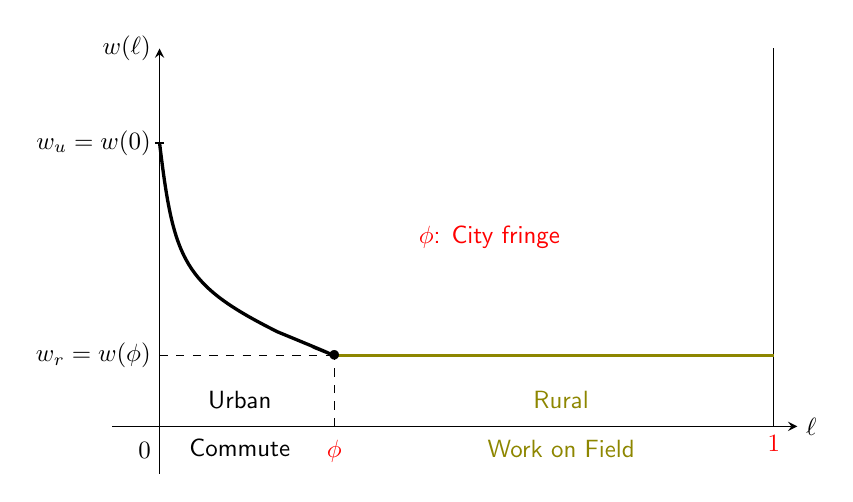
\begin{tikzpicture}[scale=0.6,every node/.style={scale=0.9}]

% xaxis
\draw[->,>=stealth,line width=0.5pt] (0,-1)--(0,8);
\draw (13.5,0) node (xaxis) [right] {$\ell$};
\draw[line width=0.5pt] (13,0)--(13,8);  % right y-axis
\draw (13,0) node [below] {\color{red}{$1$}};  % right y-axis label
\draw (0,-0.5) node (xaxis) [left] {$0$};
\draw[->,>=stealth,line width=0.5pt] (-1,0)--(13.5,0);%y axis


% axis labels

\uncover<2->{

\draw (0,8) node[left] {$w(\ell)$};  % yaxis label
% intercept of w(0)
\draw[line width=0.5pt] (-0.1,6)--(0.1,6);
\draw (0,6) node (yaxis) [left] {$w_u=w(0)$};}

\uncover<3->{
	% wage function
	\draw[line width=1.2pt, black] (0,6) ..controls +(0.3,-2.5) and +(-2,1).. (2.5,2) ..controls +(1.7,-0.7) and +(-0.5,0.2).. (3.7,1.5);
}


\uncover<4->{
% wage from phi to 1
\draw[line width=1.3pt,olive](3.7,1.5)--(13,1.5);

% dashed line for q(phi) and phi
\draw [dashed] (3.7,0) |-(3.7,1.5);
\draw [dashed] (0,1.5)--(3.7,1.5);
\draw (0,1.5) node [left] {$w_r=w(\phi)$};
\draw (3.7,1.5) node[black]{$\bullet$};
\draw (5.3,4) node[right] {\color{red}{$\phi$}\textsf{: City fringe}};
\draw (3.7,-0.1) node[below] {\color{red}{$\phi$}};

% text annotations
\draw (1.7,0.2) node[above] {\textsf{Urban}};
\draw (1.7,-0.08) node[below] {\textsf{Commute}};
\draw (8.5,0.2) node[above] {\textsf{\color{olive}{Rural}}};
\draw (8.5,-0.1) node[below] {\textsf{\color{olive}{Work on Field}}};}
\end{tikzpicture}
\end{center}

% \end{document}
% \end{column}
% \begin{column}{0.3\textwidth}
% \begin{mide}
% \item Space $\ell \in[0,1]$
% \pause
% \item Urban production at $\ell=0$
% \pause
% \item Residence at any $\ell \in[0,1]$
% \pause
% \item $\tau(\ell)$: commuting cost from $\ell$
% \pause
% \item $w_u(1-\tau(\ell))$ urban wage
% \end{mide}
% \end{column}
% \end{columns}
% \end{frame}

\begin{frame}{Spatial Structure: Wage Function $w(\ell)$}{Wages Net Of Commuting Costs in Spatial Equilibrium: $C(\ell) = \bar{U}$}
\begin{columns}
\begin{column}{0.7\textwidth}

% \documentclass[border=10pt]{standalone}
% \usepackage{tikz}
% \usepackage{stmaryrd}

% \begin{document}
\begin{center}
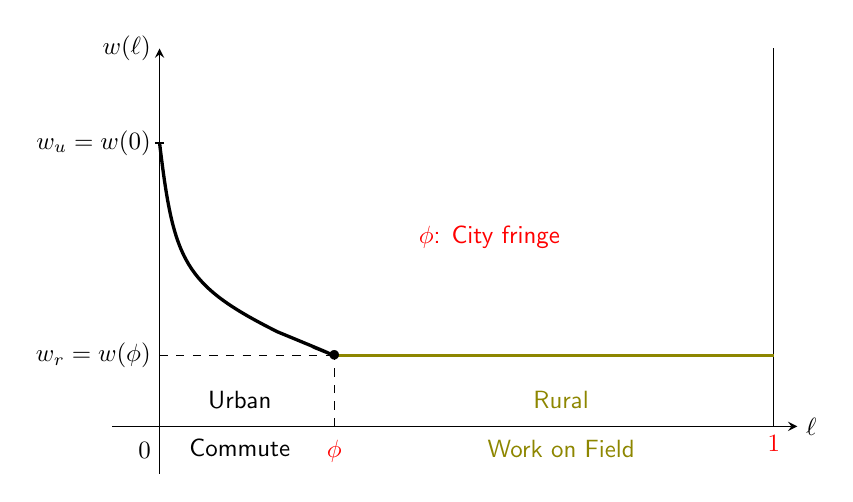
\begin{tikzpicture}[scale=0.6,every node/.style={scale=0.9}]

% xaxis
\draw[->,>=stealth,line width=0.5pt] (0,-1)--(0,8);
\draw (13.5,0) node (xaxis) [right] {$\ell$};
\draw[line width=0.5pt] (13,0)--(13,8);  % right y-axis
\draw (13,0) node [below] {\color{red}{$1$}};  % right y-axis label
\draw (0,-0.5) node (xaxis) [left] {$0$};
\draw[->,>=stealth,line width=0.5pt] (-1,0)--(13.5,0);%y axis


% axis labels

\uncover<2->{

\draw (0,8) node[left] {$w(\ell)$};  % yaxis label
% intercept of w(0)
\draw[line width=0.5pt] (-0.1,6)--(0.1,6);
\draw (0,6) node (yaxis) [left] {$w_u=w(0)$};}

\uncover<3->{
	% wage function
	\draw[line width=1.2pt, black] (0,6) ..controls +(0.3,-2.5) and +(-2,1).. (2.5,2) ..controls +(1.7,-0.7) and +(-0.5,0.2).. (3.7,1.5);
}


\uncover<4->{
% wage from phi to 1
\draw[line width=1.3pt,olive](3.7,1.5)--(13,1.5);

% dashed line for q(phi) and phi
\draw [dashed] (3.7,0) |-(3.7,1.5);
\draw [dashed] (0,1.5)--(3.7,1.5);
\draw (0,1.5) node [left] {$w_r=w(\phi)$};
\draw (3.7,1.5) node[black]{$\bullet$};
\draw (5.3,4) node[right] {\color{red}{$\phi$}\textsf{: City fringe}};
\draw (3.7,-0.1) node[below] {\color{red}{$\phi$}};

% text annotations
\draw (1.7,0.2) node[above] {\textsf{Urban}};
\draw (1.7,-0.08) node[below] {\textsf{Commute}};
\draw (8.5,0.2) node[above] {\textsf{\color{olive}{Rural}}};
\draw (8.5,-0.1) node[below] {\textsf{\color{olive}{Work on Field}}};}
\end{tikzpicture}
\end{center}

% \end{document}
\end{column}
\begin{column}{0.3\textwidth}
\begin{mide}
\item<1-> Space $\ell \in[0,1]$
\item<2-> Urban production at $\ell=0$
\item<2-> Residence at any $\ell \in[0,1]$
\item<3-> $\tau(\ell)$: commuting cost from $\ell$
\item<3-> $w_u - \tau(\ell)$ urban wage
\item<4-> {\color{red}{$\phi$}} denotes urban fringe.
\end{mide}
\end{column}
\end{columns}
\end{frame}

% \begin{frame}{Comparative Statics: Increase in Rural Productivity}

% 	\begin{columns}
% 		\begin{column}{0.7\textwidth}
% 			% \documentclass[border=10pt]{standalone}
% \usepackage{tikz}
% % \usepackage{stmaryrd}

% \begin{document}

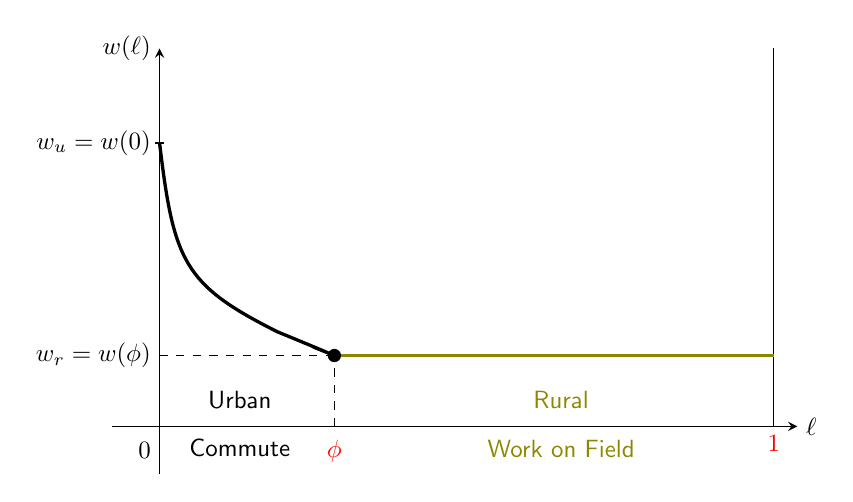
\begin{tikzpicture}[scale=0.6,every node/.style={scale=0.9}]



\pgfmathsetmacro{\WU}{6.0}
\pgfmathsetmacro{\WR}{1.5}
\pgfmathsetmacro{\PHI}{3.7}



  % xaxis
\draw[->,>=stealth,line width=0.5pt] (0,-1)--(0,8);
\draw (13.5,0) node (xaxis) [right] {$\ell$};
\draw[line width=0.5pt] (13,0)--(13,8);  % right y-axis
\draw (13,0) node [below] {\color{red}{$1$}};  % right y-axis label
\draw (0,-0.5) node (xaxis) [left] {$0$};
\draw[->,>=stealth,line width=0.5pt] (-1,0)--(13.5,0);%y axis


% axis labels

% \uncover<2->{

\draw (0,8) node[left] {$w(\ell)$};  % yaxis label
% intercept of w(0)
\draw[line width=0.5pt] (-0.1,\WU)--(0.1,\WU);
\draw (0,\WU) node (yaxis) [left] {$w_u=w(0)$};
% }

% \uncover<3->{
	% wage function
	\draw[line width=1.2pt, black] (0,\WU) ..controls +(0.3,-2.5) and +(-2,1).. (2.5,2) ..controls +(1.7,-0.7) and +(-0.5,0.2).. (\PHI,\WR);
% }


% \uncover<4->{
% wage from phi to 1
\draw[line width=1.3pt,olive](\PHI,\WR)--(13,\WR);

% dashed line for q(phi) and phi
\draw [dashed] (\PHI,0) |-(\PHI,\WR);
\draw [dashed] (0,\WR)--(\PHI,\WR);
\draw (0,\WR) node [left] {$w_r=w(\phi)$};
\fill (\PHI,\WR) circle[radius=4pt];
% \draw (5.3,4) node[right] {\color{red}{$\phi$}\textsf{: City fringe}};
\draw (\PHI,-0.1) node[below] {\color{red}{$\phi$}};

% text annotations
\draw (1.7,0.2) node[above] {\textsf{Urban}};
\draw (1.7,-0.08) node[below] {\textsf{Commute}};
\draw (8.5,0.2) node[above] {\textsf{\color{olive}{Rural}}};
\draw (8.5,-0.1) node[below] {\textsf{\color{olive}{Work on Field}}};
\end{tikzpicture}


% \end{document}
% 		\end{column}
% 		\begin{column}{0.3\textwidth}
% 			\begin{midi}
% 				\item Rural prod. $\theta_r \uparrow$
				
% 			\end{midi}
% 		\end{column}
% 		\end{columns}
	
	
% \end{frame}

% \begin{frame}{Comparative Statics: Increase in Rural Productivity}

% 	\begin{columns}
% 		\begin{column}{0.7\textwidth}
% 			% \documentclass[border=10pt]{standalone}
% \usepackage{tikz}
% % \usepackage{stmaryrd}

% \begin{document}

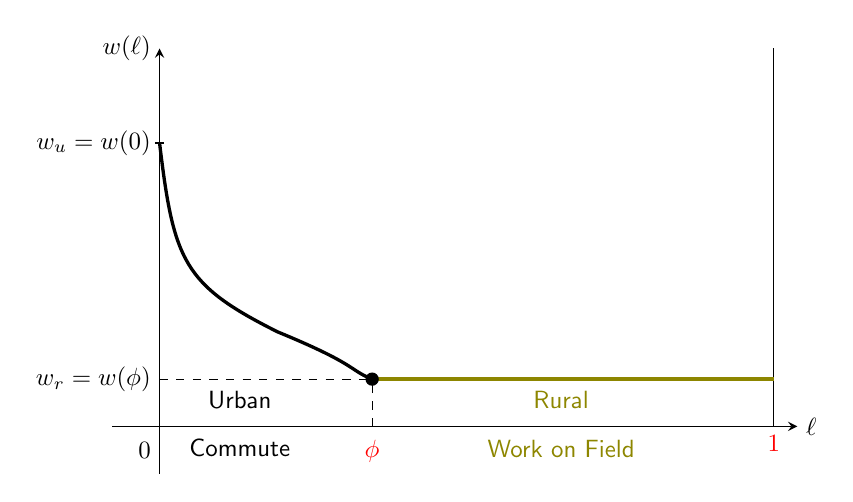
\begin{tikzpicture}[scale=0.6,every node/.style={scale=0.9}]



\pgfmathsetmacro{\WU}{6.0}
\pgfmathsetmacro{\WR}{1.0}
\pgfmathsetmacro{\PHI}{4.5}



  % xaxis
\draw[->,>=stealth,line width=0.5pt] (0,-1)--(0,8);
\draw (13.5,0) node (xaxis) [right] {$\ell$};
\draw[line width=0.5pt] (13,0)--(13,8);  % right y-axis
\draw (13,0) node [below] {\color{red}{$1$}};  % right y-axis label
\draw (0,-0.5) node (xaxis) [left] {$0$};
\draw[->,>=stealth,line width=0.5pt] (-1,0)--(13.5,0);%y axis


% axis labels

% \uncover<2->{

\draw (0,8) node[left] {$w(\ell)$};  % yaxis label
% intercept of w(0)
\draw[line width=0.5pt] (-0.1,\WU)--(0.1,\WU);
\draw (0,\WU) node (yaxis) [left] {$w_u=w(0)$};
% }

% \uncover<3->{
	% wage function
	\draw[line width=1.2pt, black] (0,\WU) ..controls +(0.3,-2.5) and +(-2,1).. (2.5,2) ..controls +(1.7,-0.7) and +(-0.5,0.2).. (\PHI,\WR);
% }


% \uncover<4->{
% wage from phi to 1
\draw[line width=1.3pt,olive](\PHI,\WR)--(13,\WR);

% dashed line for q(phi) and phi
\draw [dashed] (\PHI,0) |-(\PHI,\WR);
\draw [dashed] (0,\WR)--(\PHI,\WR);
\draw (0,\WR) node [left] {$w_r=w(\phi)$};
\fill (\PHI,\WR) circle[radius=4pt];
% \draw (5.3,4) node[right] {\color{red}{$\phi$}\textsf{: City fringe}};
\draw (\PHI,-0.1) node[below] {\color{red}{$\phi$}};

% text annotations
\draw (1.7,0.2) node[above] {\textsf{Urban}};
\draw (1.7,-0.08) node[below] {\textsf{Commute}};
\draw (8.5,0.2) node[above] {\textsf{\color{olive}{Rural}}};
\draw (8.5,-0.1) node[below] {\textsf{\color{olive}{Work on Field}}};
\end{tikzpicture}


% \end{document}
% 		\end{column}
% 		\begin{column}{0.3\textwidth}
% 			\begin{midi}
% 				\item Rural prod. $\theta_r \uparrow$
% 				\item $\theta_r \uparrow \Rightarrow (\rho_r \downarrow, w_r \downarrow)$
% 				\item Indifference point is pushed outwards.
% 			\end{midi}
% 		\end{column}
% 		\end{columns}
	
	
% \end{frame}

% \begin{frame}{Comparative Statics: Increase in Urban Productivity}

% 	\begin{columns}
% 		\begin{column}{0.7\textwidth}
% 			% \documentclass[border=10pt]{standalone}
% \usepackage{tikz}
% % \usepackage{stmaryrd}

% \begin{document}

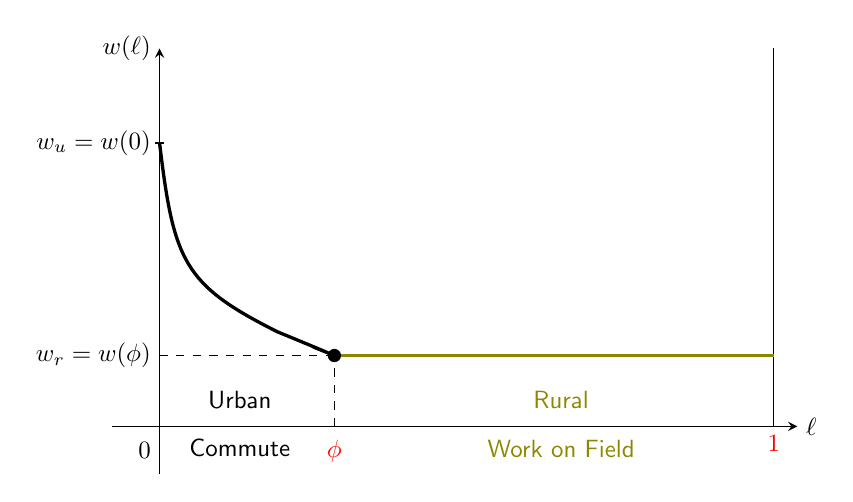
\begin{tikzpicture}[scale=0.6,every node/.style={scale=0.9}]



\pgfmathsetmacro{\WU}{6.0}
\pgfmathsetmacro{\WR}{1.5}
\pgfmathsetmacro{\PHI}{3.7}



  % xaxis
\draw[->,>=stealth,line width=0.5pt] (0,-1)--(0,8);
\draw (13.5,0) node (xaxis) [right] {$\ell$};
\draw[line width=0.5pt] (13,0)--(13,8);  % right y-axis
\draw (13,0) node [below] {\color{red}{$1$}};  % right y-axis label
\draw (0,-0.5) node (xaxis) [left] {$0$};
\draw[->,>=stealth,line width=0.5pt] (-1,0)--(13.5,0);%y axis


% axis labels

% \uncover<2->{

\draw (0,8) node[left] {$w(\ell)$};  % yaxis label
% intercept of w(0)
\draw[line width=0.5pt] (-0.1,\WU)--(0.1,\WU);
\draw (0,\WU) node (yaxis) [left] {$w_u=w(0)$};
% }

% \uncover<3->{
	% wage function
	\draw[line width=1.2pt, black] (0,\WU) ..controls +(0.3,-2.5) and +(-2,1).. (2.5,2) ..controls +(1.7,-0.7) and +(-0.5,0.2).. (\PHI,\WR);
% }


% \uncover<4->{
% wage from phi to 1
\draw[line width=1.3pt,olive](\PHI,\WR)--(13,\WR);

% dashed line for q(phi) and phi
\draw [dashed] (\PHI,0) |-(\PHI,\WR);
\draw [dashed] (0,\WR)--(\PHI,\WR);
\draw (0,\WR) node [left] {$w_r=w(\phi)$};
\fill (\PHI,\WR) circle[radius=4pt];
% \draw (5.3,4) node[right] {\color{red}{$\phi$}\textsf{: City fringe}};
\draw (\PHI,-0.1) node[below] {\color{red}{$\phi$}};

% text annotations
\draw (1.7,0.2) node[above] {\textsf{Urban}};
\draw (1.7,-0.08) node[below] {\textsf{Commute}};
\draw (8.5,0.2) node[above] {\textsf{\color{olive}{Rural}}};
\draw (8.5,-0.1) node[below] {\textsf{\color{olive}{Work on Field}}};
\end{tikzpicture}


% \end{document}
% 		\end{column}
% 		\begin{column}{0.3\textwidth}
% 			\begin{midi}
% 				\item Urban prod. $\theta_u \uparrow \Rightarrow w_u \uparrow$
% 			\end{midi}
% 		\end{column}
% 		\end{columns}
	
	
% \end{frame}

% \begin{frame}{Comparative Statics: Increase in Urban Productivity}

% 	\begin{columns}
% 		\begin{column}{0.7\textwidth}
% 			% \documentclass[border=10pt]{standalone}
% \usepackage{tikz}
% % \usepackage{stmaryrd}

% \begin{document}

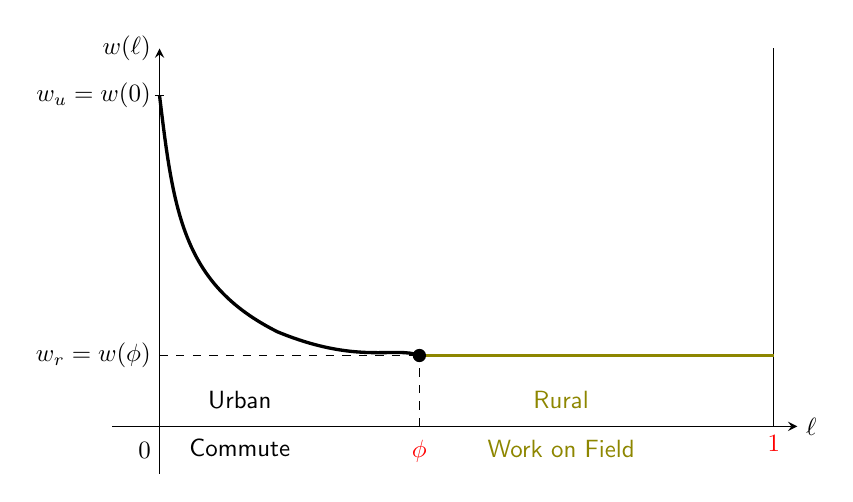
\begin{tikzpicture}[scale=0.6,every node/.style={scale=0.9}]



\pgfmathsetmacro{\WU}{7.0}
\pgfmathsetmacro{\WR}{1.5}
\pgfmathsetmacro{\PHI}{5.5}



  % xaxis
\draw[->,>=stealth,line width=0.5pt] (0,-1)--(0,8);
\draw (13.5,0) node (xaxis) [right] {$\ell$};
\draw[line width=0.5pt] (13,0)--(13,8);  % right y-axis
\draw (13,0) node [below] {\color{red}{$1$}};  % right y-axis label
\draw (0,-0.5) node (xaxis) [left] {$0$};
\draw[->,>=stealth,line width=0.5pt] (-1,0)--(13.5,0);%y axis


% axis labels

% \uncover<2->{

\draw (0,8) node[left] {$w(\ell)$};  % yaxis label
% intercept of w(0)
\draw[line width=0.5pt] (-0.1,\WU)--(0.1,\WU);
\draw (0,\WU) node (yaxis) [left] {$w_u=w(0)$};
% }

% \uncover<3->{
	% wage function
	\draw[line width=1.2pt, black] (0,\WU) ..controls +(0.3,-2.5) and +(-2,1).. (2.5,2) ..controls +(1.7,-0.7) and +(-0.5,0.2).. (\PHI,\WR);
% }


% \uncover<4->{
% wage from phi to 1
\draw[line width=1.3pt,olive](\PHI,\WR)--(13,\WR);

% dashed line for q(phi) and phi
\draw [dashed] (\PHI,0) |-(\PHI,\WR);
\draw [dashed] (0,\WR)--(\PHI,\WR);
\draw (0,\WR) node [left] {$w_r=w(\phi)$};
\fill (\PHI,\WR) circle[radius=4pt];
% \draw (5.3,4) node[right] {\color{red}{$\phi$}\textsf{: City fringe}};
\draw (\PHI,-0.1) node[below] {\color{red}{$\phi$}};

% text annotations
\draw (1.7,0.2) node[above] {\textsf{Urban}};
\draw (1.7,-0.08) node[below] {\textsf{Commute}};
\draw (8.5,0.2) node[above] {\textsf{\color{olive}{Rural}}};
\draw (8.5,-0.1) node[below] {\textsf{\color{olive}{Work on Field}}};
\end{tikzpicture}


% \end{document}
% 		\end{column}
% 		\begin{column}{0.3\textwidth}
% 			\begin{midi}
% 				\item Urban prod. $\theta_u \uparrow \Rightarrow w_u \uparrow$
% 				\item all else equal, last worker will commute longer distance.
% 			\end{midi}
% 		\end{column}
% 		\end{columns}
	
	
% \end{frame}

\begin{v75mins}
\begin{frame}{Commuting Costs in units of Numeraire Good}{Based on DeSalvo and Huq (JUE 1996)}

\begin{columns}
\begin{column}{0.5\textwidth}
\begin{midi}
\item Commuters choose best mode of transport.
\item Opportunity cost of time (i.e. wage) and location matter.
\item High urban wage $\rightarrow$ demand faster commute.
\end{midi}
\end{column}
\pause
\begin{column}{0.5\textwidth}
\begin{midi}
\item Balance marginal cost/benefit of faster mode:
\begin{equation*}
\tau(\ell) = a \times (w_u \ell)^\xi
\end{equation*}
\begin{enumerate}
\item Faster commutes for people further away.
\item Speed increases with wage (opp. cost of time).
\item Elasticity of $\tau(\ell)$ wrt wage is strictly less than unity% $\rightarrow$ people are willing to live further away as labor productivity increases.
\end{enumerate}
\end{midi}

\end{column}
\end{columns}

\end{frame}



\begin{frame}{Location Sorting}{Spatial Equilibrium}

\begin{columns}
\begin{column}{0.5\textwidth}

\begin{midi}
 \item  Indifference conditions across locations,
\begin{equation*}
 \overline{C}=C(\ell)=\kappa\frac{w(\ell)+\mathbf{r}+ \underline{s} - p\underline{c}}{q(\ell)^{\gamma}}.
\end{equation*}
\item Same house price $q_r$ at $\phi$ and in the rural area, $q(\ell \geq \phi)=q_r$.
\item Indifference at the fringe,
\begin{equation*}
\re{w(\phi)=w_u -\tau(\phi)=w_r}
\end{equation*}
\end{midi} 
\end{column}		
\pause
\begin{column}{0.5\textwidth}

	\begin{midi}
		\item The last urban worker has same net wage as rural worker.
		\item Higher commuting costs deter rural workers to move into urban sector.
	\end{midi}
	
\end{column}


% 
% \documentclass[border=10pt]{standalone}
% \usepackage{tikz}
% \usepackage{stmaryrd}

% \begin{document}
\begin{center}
\begin{tikzpicture}[remember picture,overlay]

\node[anchor=north east] at ($(current page.north east)+(0,-2.5)$) {
\begin{tikzpicture}[scale=0.45,every node/.style={scale=0.8}]

  % xaxis
\draw[->,>=stealth,line width=0.5pt] (0,-1)--(0,8);
\draw (13.5,0) node (xaxis) [right] {$\ell$};
\draw[line width=0.5pt] (13,0)--(13,8);  % right y-axis
\draw (13,0) node [below] {\color{red}{$1$}};  % right y-axis label
\draw (0,-0.5) node (xaxis) [left] {$0$};
\draw[->,>=stealth,line width=0.5pt] (-1,0)--(13.5,0);%y axis


% axis labels

% \uncover<2->{

\draw (0,8) node[left] {$w(\ell)$};  % yaxis label
% intercept of w(0)
\draw[line width=0.5pt] (-0.1,6)--(0.1,6);
\draw (0,6) node (yaxis) [left] {$w_u=w(0)$};
% }

% \uncover<3->{
	% wage function
	\draw[line width=1.2pt, black] (0,6) ..controls +(0.3,-2.5) and +(-2,1).. (2.5,2) ..controls +(1.7,-0.7) and +(-0.5,0.2).. (3.7,1.5);
% }


% \uncover<4->{
% wage from phi to 1
\draw[line width=1.3pt,olive](3.7,1.5)--(13,1.5);

% dashed line for q(phi) and phi
\draw [dashed] (3.7,0) |-(3.7,1.5);
\draw [dashed] (0,1.5)--(3.7,1.5);
\draw (0,1.5) node [left] {$w_r=w(\phi)$};
% \draw (3.7,1.5) node[black]{$\bullet$};
\draw (5.3,4) node[right] {\color{red}{$\phi$}\textsf{: City fringe}};
\draw (3.7,-0.1) node[below] {\color{red}{$\phi$}};

% text annotations
\draw (1.7,0.2) node[above] {\textsf{Urban}};
\draw (1.7,-0.08) node[below] {\textsf{Commute}};
\draw (8.5,0.2) node[above] {\textsf{\color{olive}{Rural}}};
\draw (8.5,-0.1) node[below] {\textsf{\color{olive}{Work on Field}}};
\end{tikzpicture}
% }
};


\end{tikzpicture}
\end{center}

% \end{document}
\end{columns}

\end{frame}

% \begin{frame}
% \frametitle{Equilibrium Sorting}
% \framesubtitle{Housing Rental Price Gradient}
% \bi
% \item Competition for location: $q(\ell)$ adjusts to equalize utility across locations.
% \begin{equation*}
% q(\ell)=q_r\left( \frac{w(\ell)+\mathbf{r}-p\underline{c}}{w(\phi)+\mathbf{r}-p\underline{c}}\right)
% ^{1/\gamma}=q_r\left( \frac{w(\ell)+\mathbf{r}-p\underline{c}}{w_r+\mathbf{r}-p\underline{c}}\right)
% ^{1/\gamma}.
% \end{equation*}
% \item Within the city, $q(\ell)$ is falling with $\ell$ to compensate workers who live in worse locations.
% \item In the rural area, $\ell$ above $\phi$, housing price is constant across locations, equal to $q_r$.
% \ei
% %The crucial difference compared to the standard urban model is that the price at the fringe $q$ is endogenously determined in our general equilibrium model.
% \end{frame}

% \begin{frame}
% \frametitle{Housing Market Equilibrium}
% \framesubtitle{Housing Demand}
% \bi
% \item Demand for housing space per worker in each location increasing with $\ell$ for $\ell \leq \phi$,
% \bigskip

% $h(\ell)=\gamma \left( \frac{w(\ell)+\mathbf{r}-p\underline{c}}{q(\ell)}\right)$\\
% $h(\ell)=\left(
% \frac{\gamma }{q_r}\right) (w(\phi)+\mathbf{r}-p\underline{c})^{1/\gamma}
% (w(\ell)+\mathbf{r}-p\underline{c})^{1-1/\gamma}$
% \bigskip

% %Facing higher housing prices, household closer to the CBD demand less housing space.
% \item For locations in the rural area, housing demand per rural worker is constant, $h(\ell \geq \phi)=\gamma \left( \frac{w_r+\mathbf{r}-p\underline{c}}{q_r}\right)$.
% \ei
% \end{frame}


\begin{frame}{Housing Rental Price Gradient}{Piecewise Constant Housing Price, Demand, and Population Density}
\begin{columns}
\begin{column}{0.7\textwidth}

% \documentclass[border=10pt]{standalone}
% \usepackage{tikz}
% \usepackage{stmaryrd}
% \usepackage{amssymb, amsfonts,amsmath}   % \ell

% \begin{document}
\begin{center}
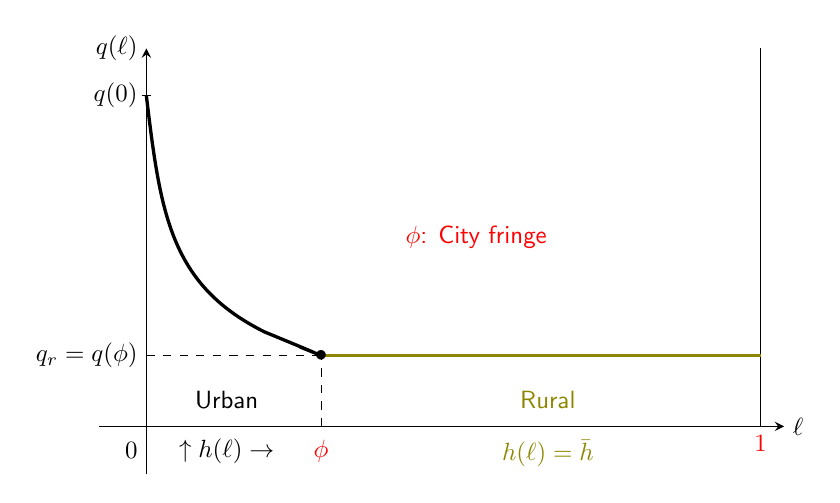
\begin{tikzpicture}[scale=0.6,every node/.style={scale=0.9}]
\draw[->,>=stealth,line width=0.5pt] (0,-1)--(0,8);
\draw[->,>=stealth,line width=0.5pt] (-1,0)--(13.5,0);
\draw (0,8) node[left] {$q(\ell)$};
\draw (13.5,0) node (xaxis) [right] {$\ell$};
\draw[line width=0.5pt] (13,0)--(13,8);  % right y-axis
\draw (13,0) node [below] {\color{red}{1}};  % right y-axis label
\draw (0,-0.5) node (xaxis) [left] {$0$};
\draw[line width=0.5pt] (-0.1,7)--(0.1,7);
\draw (0,7) node (yaxis) [left] {$q(0)$};
\draw (3.7,-0.1) node[below] {\color{red}{$\phi$}};
\draw[line width=1.2pt, black] (0,7) ..controls +(0.3,-2.5) and +(-2,1).. (2.5,2) ..controls +(1.7,-0.7) and +(-0.5,0.2).. (3.7,1.5);
\draw[line width=1.3pt,olive](3.7,1.5)--(13,1.5);
\draw (1.7,0.2) node[above] {\textsf{Urban}};
\draw (1.7,-0.08) node[below] {$ \uparrow h(\ell)\rightarrow$};
\draw (8.5,0.2) node[above] {\textsf{\color{olive}{Rural}}};
\draw (8.5,-0.1) node[below] {\color{olive}{$h(\ell) = \bar{h}$}};
\draw (5.3,4) node[right] {\color{red}{$\phi$}\textsf{: City fringe}};
\draw [dashed] (0,1.5)--(3.7,1.5);
\draw (0,1.5) node [left] {$q_r=q(\phi)$};
\draw (3.7,1.5) node[black]{$\bullet$};
\draw [dashed] (3.7,0) |-(3.7,1.5);
\end{tikzpicture}
\end{center}

% \end{document}
\end{column}
\begin{column}{0.3\textwidth}
Closed forms for:
\begin{midi}
\item House price $q(\ell)$
\item Housing demand $h(\ell)$
\item Population Density: $D(\ell)$
\end{midi}

\end{column}
\end{columns}
\end{frame}

\end{v75mins}


% \begin{frame}{Closing The Model}{Market Clearing}

% We need to clear 5 Markets in order to find:

% \begin{mide}
% \item The price of land in each location $\rho(\ell)$
% \item The number of people living in the city
% \item Urban Goods Market: Equate Urban Good Production and Consumption.
% \item Rural Goods 
% \end{mide}

% \end{frame}



\begin{v75mins}
\begin{frame}[label=landdevelopers]
\frametitle{Housing Market Equilibrium}
\framesubtitle{Land developers}
\bi
\item Housing supply provided by land developers.
\item Use more or less intensively the land for residential purposes.
\item Technology\\
\medskip
In each location, developers supply housing space $H(\ell)$ per unit of land with a convex cost,
\begin{equation*}
\frac{H(\ell)^{1+1/\epsilon}}{1+1/\epsilon},
\end{equation*}
in units of the numeraire.\\
 \re{$\epsilon=$} cost parameter, possibly dependent on the location.
    %which is meant to capture that it might be more costly for developers to build closer to the city center than in the suburbs or the rural part of the economy. but needs toe be the same at the fringe and in the rural part
\ei
\end{frame}

\begin{frame}
\frametitle{Housing Market Equilibrium}
\framesubtitle{Housing supply}
\bi
\item Profits per unit of land at $\ell$,
\begin{equation*}
\pi(\ell)=q(\ell)H(\ell)-\frac{H(\ell)^{1+1/\epsilon_{\ell}}}{ 1+1/\epsilon_{\ell} }- \rho(\ell),
\end{equation*}
$\rho(\ell)$ the price of a unit of \textbf{land} in $\ell$.
\item Housing supply from profit maximization,
\begin{equation*}
H(\ell)=q(\ell) ^{\epsilon_{\ell}},
\end{equation*}
with housing supply elasticity  $\re{\epsilon_{\ell}\geq 0}$, $\re{\partial\epsilon_{\ell}/\partial \ell \geq 0}$.

see Baum-Snow and Huan (2019).  %important quantitatively but not qualitatively
\ei
\end{frame}

\begin{frame}
\frametitle{Housing Market Equilibrium: Supply}
\framesubtitle{Land Prices and Land Use}
\bi
\item Profit maximization and free entry of developers pins down land prices in $\ell$,
\begin{equation*}
\rho(\ell)=\frac{q(\ell)^{1+\epsilon_{\ell}}}{ 1+\epsilon_{\ell}},
\end{equation*}
\item Land use with the highest rental value (\re{Rivalry})
\item Indifference conditions across uses at the fringe,
\begin{equation*}
 \re{\rho_r=\frac{\left( q_r \right)^{1+\epsilon_r}}{1+\epsilon_r} = (1-\alpha)p\theta_r\left(\frac{L_r}{S_r}\right)^{\alpha} }.
\end{equation*}
\ei
\end{frame}
\end{v75mins}


\begin{frame}{Equilibrium}

	\begin{midi}
		\item Land developers buy land and numeraire good to provide residential floorspace.
		\item Arbitrage across land use at the fringe pins down land values and house prices:
		\begin{equation*}
			\rho_r = \frac{q_r^{1+\epsilon}}{1+\epsilon} = (1-\alpha)p \theta_r \left(\frac{L_r}{S_r}\right)^\alpha
		\end{equation*}
		\item Land Market Clearing.
		\item Labour Market Clearing.
		\item Land Rents consistently defined.
	\end{midi}

\end{frame}

\begin{frame}
	\frametitle{Summary of Main Mechanisms}
	\framesubtitle{Transitory Dynamics with Rising Productivity and Falling Commuting Costs}
	
	\begin{widei}
	\item<1-> \textbf{Old Times:} Land is scarce. High values of farmland with respect to income due to low productivity (`food problem'). Very small and dense, \emph{walkable} cities.
	\item<2-> \textbf{Transition:} Agricultural productivity growth frees up labor and land for cities to expand. Urban workers use faster commuting modes. Cities getting large (in area) and much less dense \emph{without} a large increase in land values.
	\item<3-> \textbf{Recent Times:} Reallocation of factors/land use slows down. Cities expand less and land prices increase more with rising productivity. Land particularly scarse in some locations.
	\end{widei}
	\end{frame}

\begin{v75mins}

% \begin{frame}
% \frametitle{Housing Market Equilibrium}
% \framesubtitle{Housing market clearing in the city}
% \bi
% % \item Within the city, $\ell \leq \phi$, density \re{$D(\ell)$} in location $\ell$.
% \item Housing market clearing, $H(\ell)=D(\ell)h(\ell)$, leads to density
% \begin{equation*}
% D(\ell)= \frac{\rho_r}{\gamma_{\ell}}(w(\phi)+\mathbf{r}-p\underline{c}+\underline{s}) ^{-1/\gamma_{\ell} } (w(\ell)+\mathbf{r}-p\underline{c}+\underline{s})^{1/\gamma_{\ell} -1},
% \end{equation*}
% with $\gamma_{\ell}=\frac{\gamma}{1+\epsilon_{\ell}}=$ supply-adjusted housing spending share.
% \item Total urban population
% \begin{equation}
% \re{L_u=\int_0^{\phi}D(\ell)d\ell}  \label{eq:citysize}
% \end{equation}
% \item Pins down the city size $\phi$ for a given sectoral allocation of workers (and for given prices), \re{$\phi(L_u, w_u, \rho_r, p\underline{c})$}.
% \ei
% \end{frame}

% \begin{frame}
% \frametitle{Land and Labor Market Clearing}
% \bi
% \item Land market clearing
%  \begin{equation*}
%  \re{\phi+S_{hr}+S_r =1},
%  \end{equation*}
% with $S_{hr}=$ the land demand for housing in the rural area.
% \begin{equation*}
% S_{hr}=\frac{L_r \gamma_r \left( w_r+\mathbf{r}-p\underline{c} +\underline{s}\right)}{ \rho_r}
%  \end{equation*}
% with $\gamma_r=\gamma_\phi$ (homogenous rural housing supply conditions).
%  \item Labor market clearing
%   \begin{equation*}
%  L_u+L_r=L.
%  \end{equation*}
%  \item Land Rents
%   \begin{equation}
%  \mathbf{r} L=\int_{0}^{\phi}\rho(\ell)d\ell+\rho_r \times (1-\phi). \label{eq:landrents}
%  \end{equation}
%  \ei
% \end{frame}


% \begin{frame}
% \frametitle{Goods Market Equilibrium}
% \framesubtitle{Goods Market Clearing}
% \bi
% \item Per capita consumption of the goods, $c_i=\frac{1}{L}\int_{0}^{1}c_i(\ell)d\ell$.
% \item Per capita market clearing condition for the rural good,
% \begin{equation*}
% c_r=y_r,
% \end{equation*}
% where $y_r=\frac{Y_r}{L}=$ production per worker of $(r)$.
% \item For the urban good,
% \begin{equation*}
% c_u+\frac{w_u}{L}\int_{0}^{\phi}\tau(\ell)D(\ell)d\ell+\frac{1}{L}\int_{0}^{\phi} \frac{\epsilon_{\ell}}{1+\epsilon_{\ell}}q(\ell)H(\ell)d\ell=y_u,
% \end{equation*}
% where $y_u=\frac{Y_u}{L}=$ production per worker of $(u)$.
% \ei
% \end{frame}

% \begin{frame}
% \frametitle{Equilibrium Allocation}
% \framesubtitle{Definition of the Equilibrium}
% For technology parameters $(\theta_u,\theta_r, \alpha, \sigma)$, spatial frictions $\mathbf{\{\tau(\ell)\}_{\ell}}$, housing supply conditions $\mathbf{\{\epsilon_{\ell}\}_{\ell}}$, and preference parameters, $(\nu,\gamma, \underline{c}, \underline{s})$, an equilibrium is a sectoral labor allocation $(L_u,L_r)$, a city fringe ($\phi$) and rural land for production $(S_r)$, factors and goods prices $(w_u,w_r,\rho_r,p)$ and land rents ($\mathbf{r}$), such that:

% \emph{
% 	\begin{itemize}
% 		\item Factors are paid their marginal productivity.
% 		\item Workers are indifferent across locations.
% 		\item The demand for urban land (or city fringe $\phi$) satisfies the city size Eq. \ref{eq:citysize}.
% 		\item Land and labor markets clear.
% 	    \item Rural and urban goods markets clear.
% 		\item Land rents satisfy Eq. \ref{eq:landrents}.
	
% 	\end{itemize}
% }
% \end{frame}
\end{v75mins}

\separator{Results}


\subsection{Parameterization}


\begin{v75mins}
\begin{frame}{Numerical Illustration: Identical Growth (1.25\%) in Both Sectors}

	\begin{adjustbox}{center}
		\includegraphics[width=\textwidth]{\modelplots/baseline-6panel.png}
	\end{adjustbox}
	
\end{frame}

\begin{frame}{Numerical Illustration: Only Rural Growth}
\begin{figure}
	
	\begin{subfigure}[t]{0.32\textwidth}
		\begin{centering}
			\includegraphics[scale=0.4]{\modelplots/CitySize_agrowth.pdf}
			\caption{Urban Populatian and Area}
		\end{centering}
	\end{subfigure}
	\hfill
	\begin{subfigure}[t]{0.32\textwidth}
		\begin{centering}
			\includegraphics[scale=0.4]{\modelplots/UrbDens_agrowth.pdf}
			\caption{Urban Densities}
		\end{centering}
	\end{subfigure}
	\hfill
	\begin{subfigure}[t]{0.32\textwidth}
		\begin{centering}
			\includegraphics[scale=0.4]{\modelplots/FarmlandPrice_agrowthcomp.pdf}\end{centering}
			\caption{Farmland Price}
	\end{subfigure}
\end{figure}
\end{frame}

\begin{frame}{Numerical Illustration: Only Urban Growth}
	\begin{figure}
		
		\begin{subfigure}[t]{0.32\textwidth}
			\begin{centering}
				\includegraphics[scale=0.4]{\modelplots/CitySize_ugrowthcomp.pdf}
				\caption{Urban Populatian and Area}
			\end{centering}
		\end{subfigure}
		\hfill
		\begin{subfigure}[t]{0.32\textwidth}
			\begin{centering}
				\includegraphics[scale=0.4]{\modelplots/UrbDens_ugrowth.pdf}			
				\caption{Urban Densities}
			\end{centering}
		\end{subfigure}
		\hfill
		\begin{subfigure}[t]{0.32\textwidth}
			\begin{centering}
				\includegraphics[scale=0.4]{\modelplots/LandRents_ugrowth.pdf}
				\caption{Land rents over income}
			\end{centering}
		\end{subfigure}
	\end{figure}
	\end{frame}


\begin{frame}{Full Quantitative Model and Parameterization}
	\begin{midi}
		\item Extend the model to bring closer to the data.
		\item We estimate the $\theta$ series from data.
		\item Observed Population Growth.
		\item We use individual commuting data to calibrate $\tau$ parameters.
		\item Jointly estimate preference parameters to match set of moments.
	\end{midi}
\end{frame}

\begin{frame}{Estimated $\theta$'s}
	\begin{adjustbox}{center}
		\includegraphics[width=0.8\textwidth]{\paperroot/Thetalong_FRA1840.pdf}

		% \includegraphics[width=\textwidth]{\modelplots/smoothed-thetas.pdf}	
	\end{adjustbox}
\end{frame}

\begin{frame}{Estimation and Identification}
	We target the following moments:\medskip
	\begin{midi}
		\item $L_{rt} / L_t$: employment share in each period.
		\item City is 18\% of rural area in 2015.
		\item spending share on housing 1900 and 2010.
	\end{midi}
\vspace{1cm}
Internal city structure, density fall, commuting speed, house price: not targeted!

	
\end{frame}

\end{v75mins}

\begin{frame}{Numerical Model Results: Structural Change}

	\begin{figure}[t]
		\centering
		\makebox[0pt][c]{%
		\begin{minipage}[b]{0.36\linewidth}
				\centering
				\includegraphics[width=\textwidth]{\modelplots/AgrEmpl_data.pdf}
				\caption{Rural Employment}
			\end{minipage}%
			\begin{minipage}[b]{0.36\linewidth}
				\centering
				\includegraphics[width=\textwidth]{\modelplots/AgrPrice_data.pdf}
				\caption{$r$-good price}
			\end{minipage}%
			\begin{minipage}[b]{0.36\linewidth}
				\centering
				\includegraphics[width=\textwidth]{\modelplots/Expshares_data.pdf}
				\caption{Spending Shares}
			\end{minipage}%
		}
	\end{figure}
\end{frame}

\begin{frame}{Numerical Model Results: Urban Expansion}
	\begin{figure}[t]
		\centering
		\makebox[0pt][c]{%
		\begin{minipage}[b]{0.5\linewidth}
				\centering
				\includegraphics[width=\textwidth]{\modelplots/CitySize_data.pdf}
				\caption{City Size}
			\end{minipage}%
			\begin{minipage}[b]{0.5\linewidth}
				\centering
				\includegraphics[width=\textwidth]{\modelplots/AvgDensb_data.pdf}
				\caption{Avg. urban density}
			\end{minipage}%
		}
	\end{figure}
\end{frame}

\begin{frame}{Numerical Model Results: Urban Structure}

	\begin{figure}[t]
		\centering
		\makebox[0pt][c]{%
		\begin{minipage}[b]{0.5\linewidth}
				\centering
				\includegraphics[width=\textwidth]{\modelplots/UrbDens.pdf}
				\caption{Urban Density}
			\end{minipage}%
			\begin{minipage}[b]{0.5\linewidth}
				\centering
				\includegraphics[width=\textwidth]{\modelplots/DecDensity.pdf}
				\caption{Density Gradient (2015)}
			\end{minipage}%
		}
	\end{figure}
\end{frame}

\begin{frame}{Numerical Model Results: Commuting Speed}

	\begin{figure}[t]
		\centering
		
				\includegraphics[width=0.65\textwidth]{\modelplots/CommSpeed_data.pdf}
				\caption{Commuting Speed}
			
	\end{figure}
\end{frame}

\begin{frame}{Numerical Model Results: Wealth Distribution and House Price}

	\begin{figure}[t]
		\centering
		\makebox[0pt][c]{%
		\begin{minipage}[b]{0.5\linewidth}
				\centering
				\includegraphics[width=\textwidth]{\modelplots/WealthValues_data2.pdf}
				\caption{Urban and Rural Wealth}
			\end{minipage}%
			\begin{minipage}[b]{0.5\linewidth}
				\centering
				\includegraphics[width=\textwidth]{\modelplots/HouseIndex.pdf}
				\caption{Real House Price Index}
			\end{minipage}%
		}
	\end{figure}
\end{frame}

\begin{frame}{Extensions}

	\begin{mide}
		\item Agglomeration and Congestion.
		\item Relaxing Monocentricity.
		\item Multiple Cities.
	\end{mide}
\end{frame}


\begin{frame}{Multiple Cities}

\begin{midi}
\item Larger cities are denser than smaller cities in the cross section.
\item Over time, however, large cities get less dense at a faster rate.
\item Our model can reproduce the French cross section of cities over time.

\end{midi}
\end{frame}

\begin{frame}{Multiple Cities}{A \emph{Country} with $K$ \emph{Regions}}
\begin{widei}
\item Split total area into $K$ equal parts. (arbitrary)
\item Assume that rural productivity $\theta_{r,k}=\theta_{r}, \forall k$.
\item Initial level and growth of urban productivity $\theta_{u,k}$ determines city sizes.

\end{widei}
\end{frame}

\begin{frame}{\emph{French Top 20} Population Evolution relative to Paris}

	\begin{adjustbox}{center}
		\includegraphics[width=0.8\textwidth]{\modelplots/k20-relpop-model-data.pdf}
	\end{adjustbox}


\end{frame}

\begin{frame}{\emph{French Top 20}}

	\begin{adjustbox}{center}
		\includegraphics[width=0.8\textwidth]{\modelplots/k20-density3D.pdf}
	\end{adjustbox}

\end{frame}

\begin{frame}{\emph{French Top 20}}

	\begin{adjustbox}{center}
		\includegraphics[width=0.8\textwidth]{\modelplots/k20-xsect-time.pdf}
	\end{adjustbox}

\end{frame}



\begin{frame}
\frametitle{Conclusion}

\bi
\item Spatial general equilibrium of land use to explain
\smallskip

\bi\item The evolution of the sectoral allocation of economic activity across space.
\smallskip
\item The evolution of the density of settlements.
\smallskip
\item The evolution of the distribution of land values.
\ei
\bigskip
\item Beyond positive implications, a potentially useful tool to evaluate the welfare effects of land use restrictions.\ei

\bigskip
\begin{center}
  THANK YOU!
\end{center}
\end{frame}

\beginbackup

% \begin{frame}[label=SatParis]
% \frametitle{The area of cities}
% \framesubtitle{Satellite measurement of Paris in 2015}
% \begin{figure}
% 	\begin{center}
% 	\includegraphics[height=0.65\textheight]{\imgs/SMOD_Paris.png}
% 	\end{center}
% \end{figure}
% \hyperlink{AreaMeasure}{\beamergotobutton{back}}\\
% \end{frame}



\begin{frame}[label=LandUseMeasureParis]
	\frametitle{Land Use outside Paris 2020}
	\begin{figure}
		\begin{center}
			\includegraphics[height=0.8\textheight]{\dataplots/CLC-Paris.pdf}
		\end{center}
	\end{figure}
	\hspace{-1cm}
	\hyperlink{CLCmeasure}{\beamergotobutton{back}}\\
\end{frame}

\begin{frame}[label=LandUseMeasureLyon]
	\frametitle{Land Use outside Lyon 2020}
	\begin{figure}
		\begin{center}
			\includegraphics[height=0.8\textheight]{\dataplots/CLC-Lyon.pdf}
		\end{center}
	\end{figure}
	\hspace{-1cm}
	\hyperlink{CLCmeasure}{\beamergotobutton{back}}\\
\end{frame}

\begin{frame}[label=LandUseMeasureMarseille]
	\frametitle{Land Use outside Marseille 2020}
	\begin{figure}
		\begin{center}
			\includegraphics[height=0.8\textheight]{\dataplots/CLC-Marseille.pdf}
		\end{center}
	\end{figure}
	\hspace{-1cm}
	\hyperlink{CLCmeasure}{\beamergotobutton{back}}\\
\end{frame}

\begin{frame}[label=LandUseMeasureBordeaux]
	\frametitle{Land Use outside Bordeaux 2020}
	\begin{figure}
		\begin{center}
			\includegraphics[height=0.8\textheight]{\dataplots/CLC-Bordeaux.pdf}
		\end{center}
	\end{figure}
	\hspace{-1cm}
	\hyperlink{CLCmeasure}{\beamergotobutton{back}}\\
\end{frame}

\begin{frame}[label=violins]
\frametitle{The historical fall in urban density}
	\begin{center}
		\includegraphics[height=0.85\textheight]{\dataplots/densities-violins.pdf}
	\end{center}
\hyperlink{density}{\beamergotobutton{back}}
\end{frame}

\begin{frame}[label=Top5]
\frametitle{The historical fall in urban density}
	\begin{center}
		\includegraphics[height=0.85\textheight]{\dataplots/densities-time-top5then-city.pdf}
	\end{center}
\hyperlink{density}{\beamergotobutton{back}}
\end{frame}

\begin{frame}[label=Lyon]
\frametitle{The historical fall in urban density}
\framesubtitle{Lyon}
\begin{figure}
	\begin{center}
		\includegraphics[scale=0.65]{\imgs/logdensity_lyon.pdf}
	\end{center}
\end{figure}
\hyperlink{density}{\beamergotobutton{back}}\\
{\tiny Source: Carte Etat-Major, IGN and GHSL. Census}
\end{frame}

\begin{frame}[label=Marseille]
\frametitle{The historical fall in urban density}
\framesubtitle{Marseille}
\begin{figure}
	\begin{center}
		\includegraphics[scale=0.65]{\imgs/logdensity_marseille.pdf}
	\end{center}
\end{figure}
\hyperlink{density}{\beamergotobutton{back}}\\
{\tiny Source: Carte Etat-Major, IGN and GHSL. Census}
\end{frame}

\begin{frame}[label=Reims]
\frametitle{The historical fall in urban density}
\framesubtitle{Reims}
\begin{figure}
	\begin{center}
		\includegraphics[scale=0.65]{\imgs/logdensity_reims.pdf}
	\end{center}
\end{figure}
\hyperlink{density}{\beamergotobutton{back}}\\
{\tiny Source: Carte Etat-Major, IGN and GHSL. Census}
\end{frame}

\begin{frame}[label=world_sample_city]
\frametitle{The fall in urban density across the globe, 1990-2015}
\framesubtitle{World sample of large cities}
\begin{figure}
	\begin{center}
		\includegraphics[scale=0.6]{\imgs/worldcity_density.pdf}
	\end{center}
\end{figure}
{\tiny Source: Atlas of Urban Expansion. Sample of 73 cities above 1 000 000 people. Details in Angel et al. (2010).}\\
\hyperlink{density}{\beamergotobutton{back}}
\end{frame}

% \begin{frame}[label=sens_pref]
% \frametitle{Preferences}
% \framesubtitle{Sensitivity}
% \bi
% \item Different income elasticity of demand across goods.
% \bigskip
% \item Kongsamut, Rebelo and Xie (2001).
% \bigskip
% \item Preferences
% \begin{equation*}
% C(\ell)=\left( c_r(\ell)-\re{\underline{c}}\right)^{\nu(1-\gamma)} (c_u(\ell)+\re{\underline{s}}) ^{(1-\nu)(1-\gamma)}h(\ell)^\gamma
% \end{equation*}
% \ei
% \hyperlink{preference}{\beamergotobutton{back}}
% \end{frame}
%\small{Sensitivity. $C(\ell)=\left( c_r(\ell)-\re{\underline{c}}\right)^{\nu(1-\gamma)} (c_u(\ell)+\re{s}) ^{(1-\nu)(1-\gamma)}h(\ell)^\gamma$.}

% \begin{frame}[label=comics]
% \frametitle{Housing Market Equilibrium}
% \framesubtitle{Land Developers}
% \begin{figure}
% 	\begin{center}
% 		\includegraphics[scale=0.60]{\imgs/comics.pdf}
% 	\end{center}
% \end{figure}
% \hyperlink{landdevelopers}{\beamergotobutton{back}}
% \end{frame}

% \begin{frame}[label=comppartial]
% \frametitle{Comparative statics}
% \framesubtitle{Partial Eq. vs. GE}
% \begin{figure}
% 	\begin{center}
% 		\includegraphics[scale=0.7]{\imgs/compstat_partial_work.pdf}
% 	\end{center}
% \end{figure}
% \hyperlink{eqcharac}{\beamergotobutton{back}}
% \end{frame}

% \begin{frame}[label=comprod]
% \frametitle{Comparative statics}
% \framesubtitle{Rising Productivity}
% \begin{figure}
% 	\begin{center}
% 		\includegraphics[scale=0.7]{\imgs/compstat_prod.pdf}
% 	\end{center}
% \end{figure}
% \hyperlink{eqcharac}{\beamergotobutton{back}}
% \end{frame}

% \begin{frame}[label=compcommute]
% \frametitle{Comparative statics}
% \framesubtitle{Commuting costs, lower $\tau$}
% \begin{figure}
% 	\begin{center}
% 		\includegraphics[scale=0.7]{\imgs/compstat_tau.pdf}
% 	\end{center}
% \end{figure}
% \hyperlink{eqcharac}{\beamergotobutton{back}}
% \end{frame}

% \begin{frame}[label=compepsilon]
% \frametitle{Comparative statics}
% \framesubtitle{Housing supply conditions, higher $\epsilon$}
% \begin{figure}
% 	\begin{center}
% 		\includegraphics[scale=0.7]{\imgs/compstat_epsilon.pdf}
% 	\end{center}
% \end{figure}
% \hyperlink{eqcharac}{\beamergotobutton{back}}
% \end{frame}



%\begin{frame}[label=res_laborland_epsilon]
%\frametitle{Results}
%\framesubtitle{Labor Allocation and Land Use}
%
%1/ Share of workers in the rural sector (in green) together with land use for agriculture (braun)\\
%2/ City size (in blue)
%
%\begin{figure}
%% \label{fig:1}
%\begin{center}
%%\includegraphics[scale=0.7]{PikettyWealth_FRA.pdf}
%\end{center}
%\end{figure}
%\small{Left-panel: Share of rural workers [left-axis] and share of land in agriculture [right-axis]. Right-panel: Urban area (share of total land).}\\
%{\tiny Note: $\epsilon_{\ell}$, $\epsilon_{\phi}=4$, constant $\tau$, L=1.}\\
%\hyperlink{res_laborland}{\beamergotobutton{back}}
%\end{frame}


%\begin{frame}[label=res_density_epsilon]
%\frametitle{Results}
%\framesubtitle{Urban Density}
%
% 1/ average density (red)\\
% 2/CBD density (red) and fringe density. Large scale all the way to zero for both. Increase the scale for the fringe (up to 15?) such that it is below the CBD.
%
%\begin{figure}
%%\caption{}
%% \label{fig:1}
%\begin{center}
%%Urban Density
%%\includegraphics[scale=0.7]{PikettyWealth_FRA.pdf}
%\end{center}
%\end{figure}
%\small{Left-panel: Average Urban Density. Right-panel: Density at $\ell=0$ [left-axis] and at the fringe, $\ell=\phi$ [right-axis].}\\
%{\tiny Note: $\epsilon_{\ell}$, $\epsilon_{\phi}=4$, constant $\tau$, L=1.}\\
%\hyperlink{res_density}{\beamergotobutton{back}}
%\end{frame}

%
%\begin{frame}[label=res_landrents_epsilon]
%\frametitle{Results}
%\framesubtitle{Land Rents}
%
%1/ Aggregate land rents index (urban and all, 1990=100)\\
%2/ Land real rental prices at CBD (blue) and fringe (braun)
%
%\begin{figure}
%%\caption{}
%% \label{fig:1}
%\begin{center}
%%Land Rents
%%\includegraphics[scale=0.7]{PikettyWealth_FRA.pdf}
%\end{center}
%\end{figure}
%\small{Left-panel: Real Land Rents Index (1990=100). Right-panel: Land real rental prices at $\ell=0$  [left-axis] and at the fringe, $\ell=\phi$ [right-axis].}\\
%{\tiny Note: $\epsilon_{\ell}$, $\epsilon_{\phi}=4$, constant $\tau$, L=1.}\\
%\hyperlink{res_landrents}{\beamergotobutton{back}}
%\end{frame}



%\begin{frame}[label=res_agp_epsilon]
%\frametitle{Results}
%\framesubtitle{Urban/Rural Gap}
%
%graphs with 1/AGP 2/ ratio of housing prices at the CBD and at the fringe
%
%\begin{figure}
%%\caption{}
%% \label{fig:1}
%\begin{center}
%%Rural/Urban Wage Gap
%%\includegraphics[scale=0.7]{PikettyWealth_FRA.pdf}
%\end{center}
%\end{figure}
%\small{Left-panel: Agricultural Productivity Gap, $w_u/w_r$. Right-panel: Ratio of Housing prices at $\ell=0$ and at the fringe ($\ell=\phi$), $q(0)/q(\phi)$.}\\
%{\tiny Note: $\epsilon_{\ell}$, $\epsilon_{\phi}=4$, constant $\tau$, L=1.}\\
%\hyperlink{res_agp}{\beamergotobutton{back}}
%\end{frame}


\backupend
\end{document}





